\input{../common}
\subtitle{Lecture 1: Introduction and Version Control}

\begin{document}

\begin{frame}
  \titlepage
\end{frame}

\section{Introduction}

\begin{frame}{Programming Techniques 2026--2027}
  \begin{itemize}
    \item Lecturer: Hannu Parviainen (ULL, IAC)
    \item Language: English
    \item Contact: \texttt{hparviai@ull.edu.es}
    \item Schedule: Mondays and Wednesdays 15:00--17:00
    \item Dates: 16 September -- November 2026
    \item Location: CCA
    \item Structure: theory + exercises
    \item Reading: Fortran book, Pro Git, old lecture notes
  \end{itemize}
\end{frame}

\begin{frame}{Programming Techniques 2026--2027}
	\begin{block}{Assessment options:}
		\begin{enumerate}
			\item Two equally weighted exercises, no final exam
			\begin{itemize}
				\item Both exercises can be done over the period of several weeks
				\item GitHub is used to follow and return the exercises, as well as to discuss and share ideas
				\item Scoring is detailed separately for each exercise. However, the main criteria are that the code works, is readable and is well-documented. Interaction and involvement in GitHub is also important.
			\end{itemize}
			\vspace{0.25cm}
			\item Final exam: writing a fully working parallelised Fortran program in 4 h (paper + pen)
			\begin{itemize}
				\item Nobody has ever chosen this
			\end{itemize}
		\end{enumerate}
	\end{block}
\end{frame}


\begin{frame}{Course Topics}
  \begin{itemize}
  	\item Programming techniques in astronomy and astrophysics
    \item Modern Fortran
      \begin{itemize}
        \item Data types
        \item Flow control structures
        \item Modules, subroutines and functions
        \item Dynamic memory management (allocatable arrays, pointers)
        \item Data structures: linked lists and trees
      \end{itemize}
    \item Parallelisation: OpenMP
    \item Distributed computing: MPI
    \item Version control: Git + GitHub
    \item Makefiles
  \end{itemize}
\end{frame}


\begin{frame}{Not Course Topics}
	\begin{block}{IDEs}
	\begin{itemize}
		\item Course teaches programming, not how to use a specific Integrated Development Environment
		\item The code can be written using a text editor and compiled using command-line commands
		\item \ldots however, a good IDE can make the course way less painful
		\item Good options: \href{https://code.visualstudio.com}{VSCode} (with the \emph{Modern Fortran} extension and the \texttt{fortls} language server), \href{https://www.codeblocks.org/}{Code::Blocks}, Emacs (old-school)
		\item Check the list from \href{https://fortran-lang.org/learn/os_setup/ides/}{fortran-lang.org}
	\end{itemize}
	\end{block}
\end{frame}


\begin{frame}{Lecturer: Hannu Parviainen}
	\begin{columns}[c]
		\column{0.6\textwidth}
		\begin{itemize}
			\item Research: exoplanets, Bayesian statistics, scientific computing, radiative transfer
			\item BASIC, PASCAL, C, and C++ 1991--2004
			\item Fortran as main language 2004--2017
			\item Now: Python + Numba + OpenCL + JAX
			\item Offices at IAC and ULL
		\end{itemize}
		\column{0.35\textwidth}
		\centering
		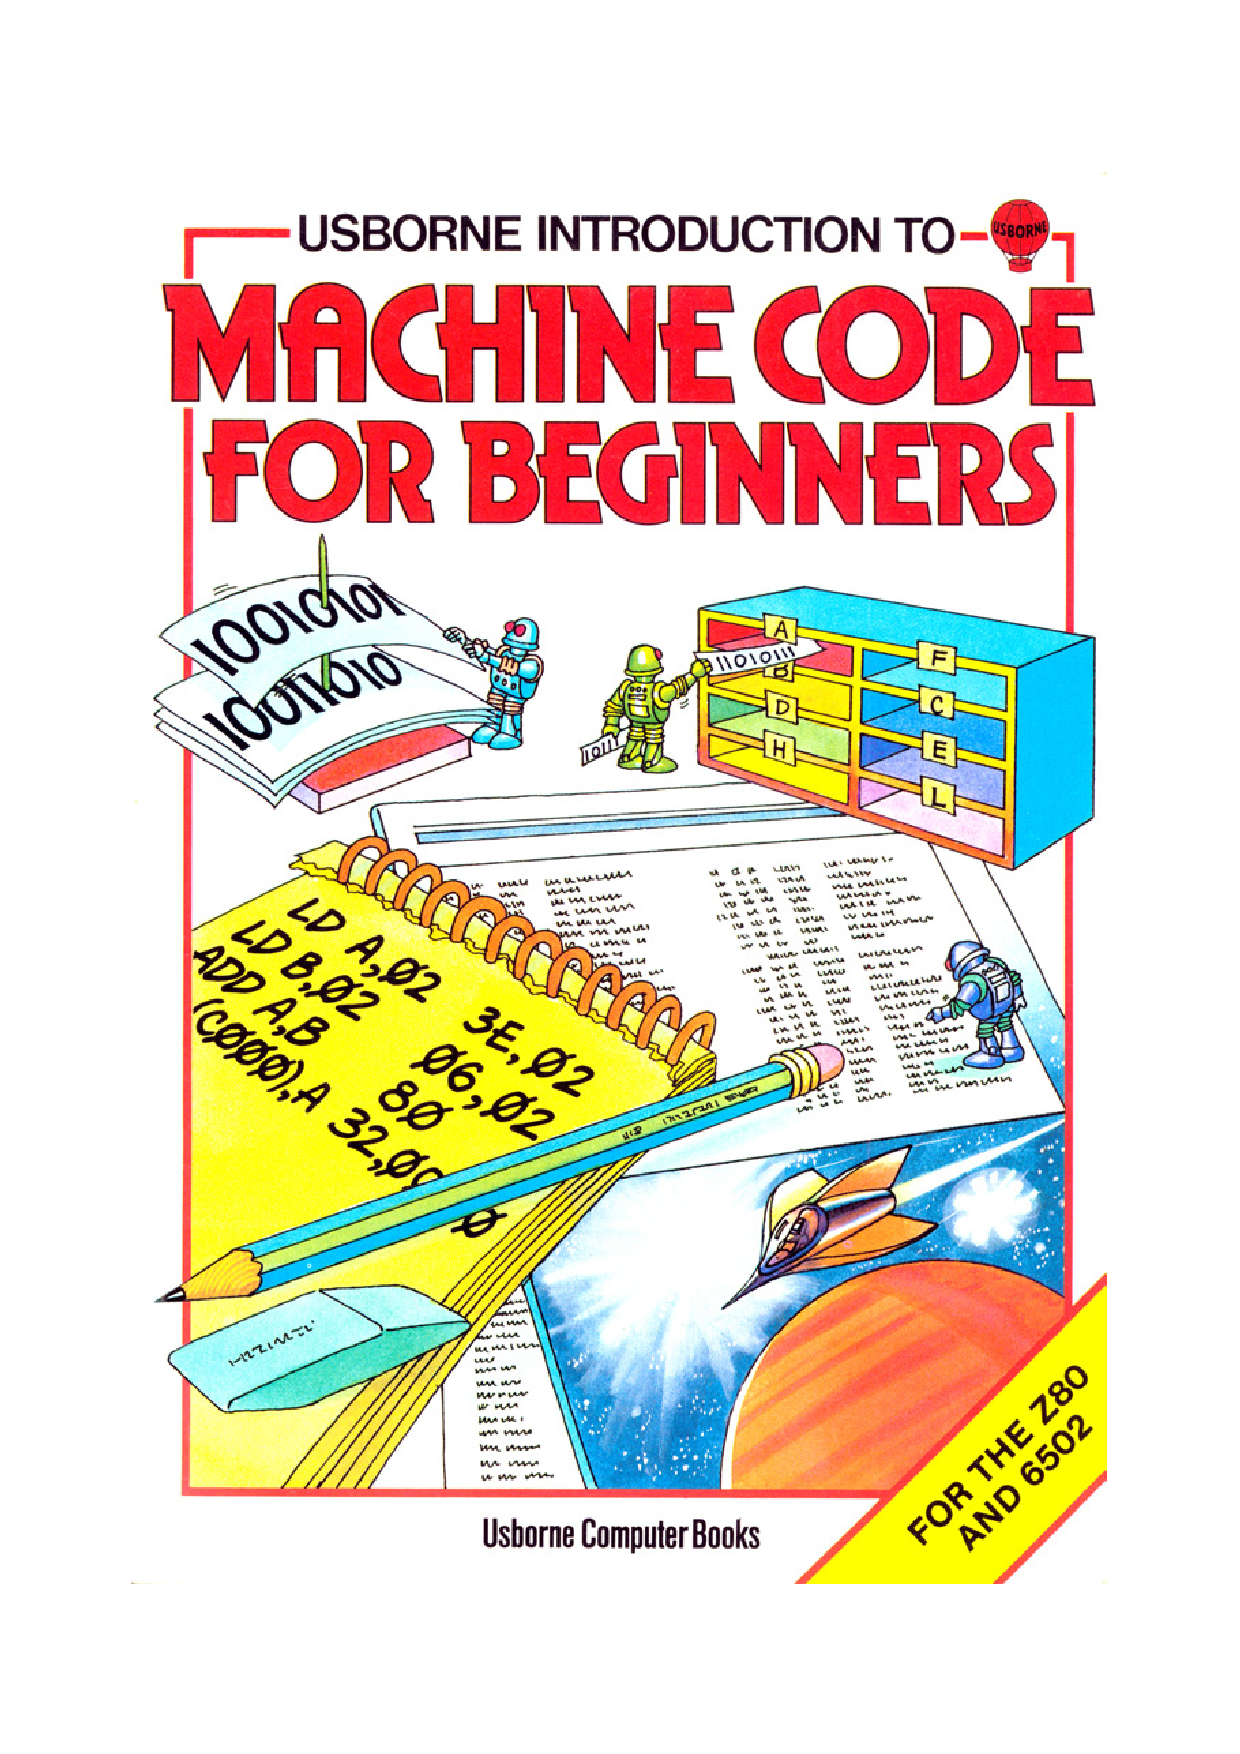
\includegraphics[height=0.8\textheight]{machine_code_for_beginners}
	\end{columns}
\end{frame}

\begin{frame}{}
	\centering
	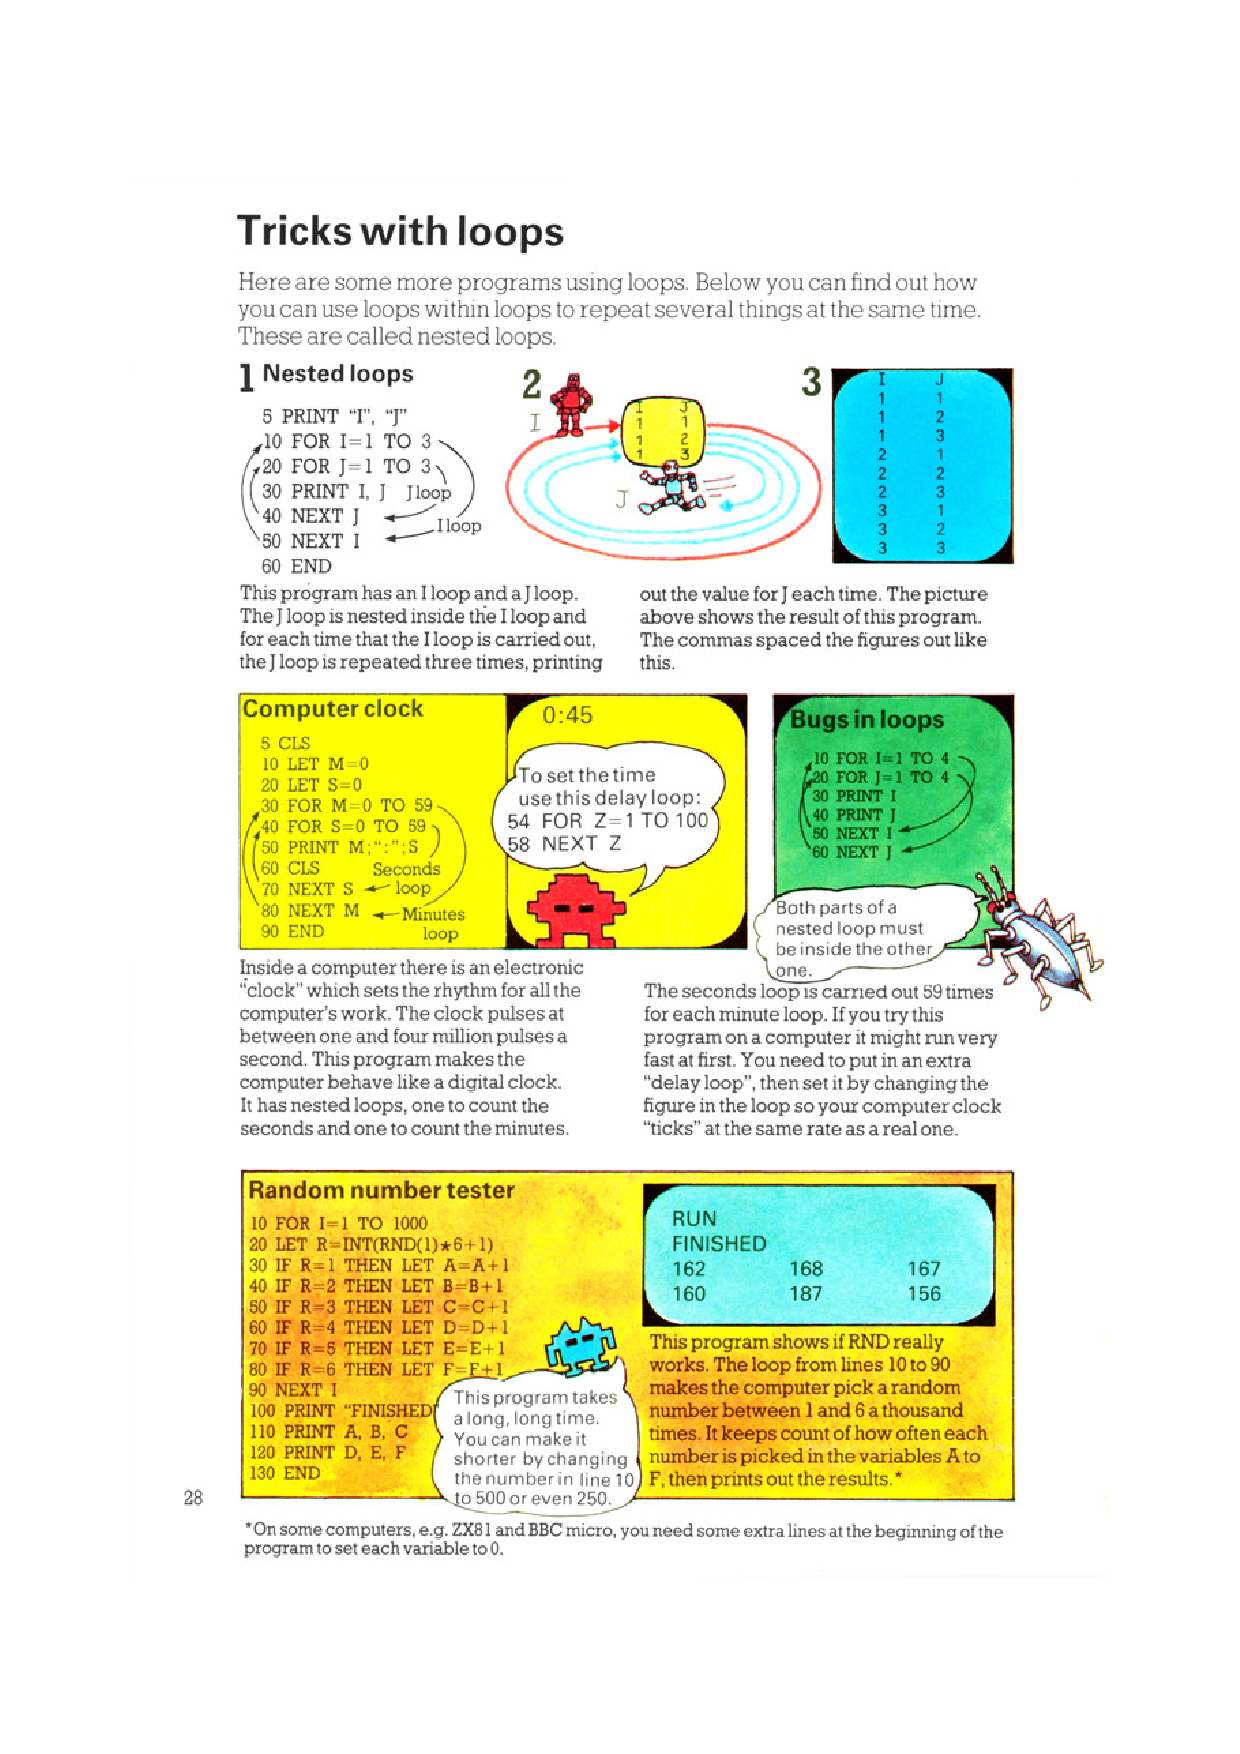
\includegraphics[height=\textheight]{loops}
	\hspace{1em}
	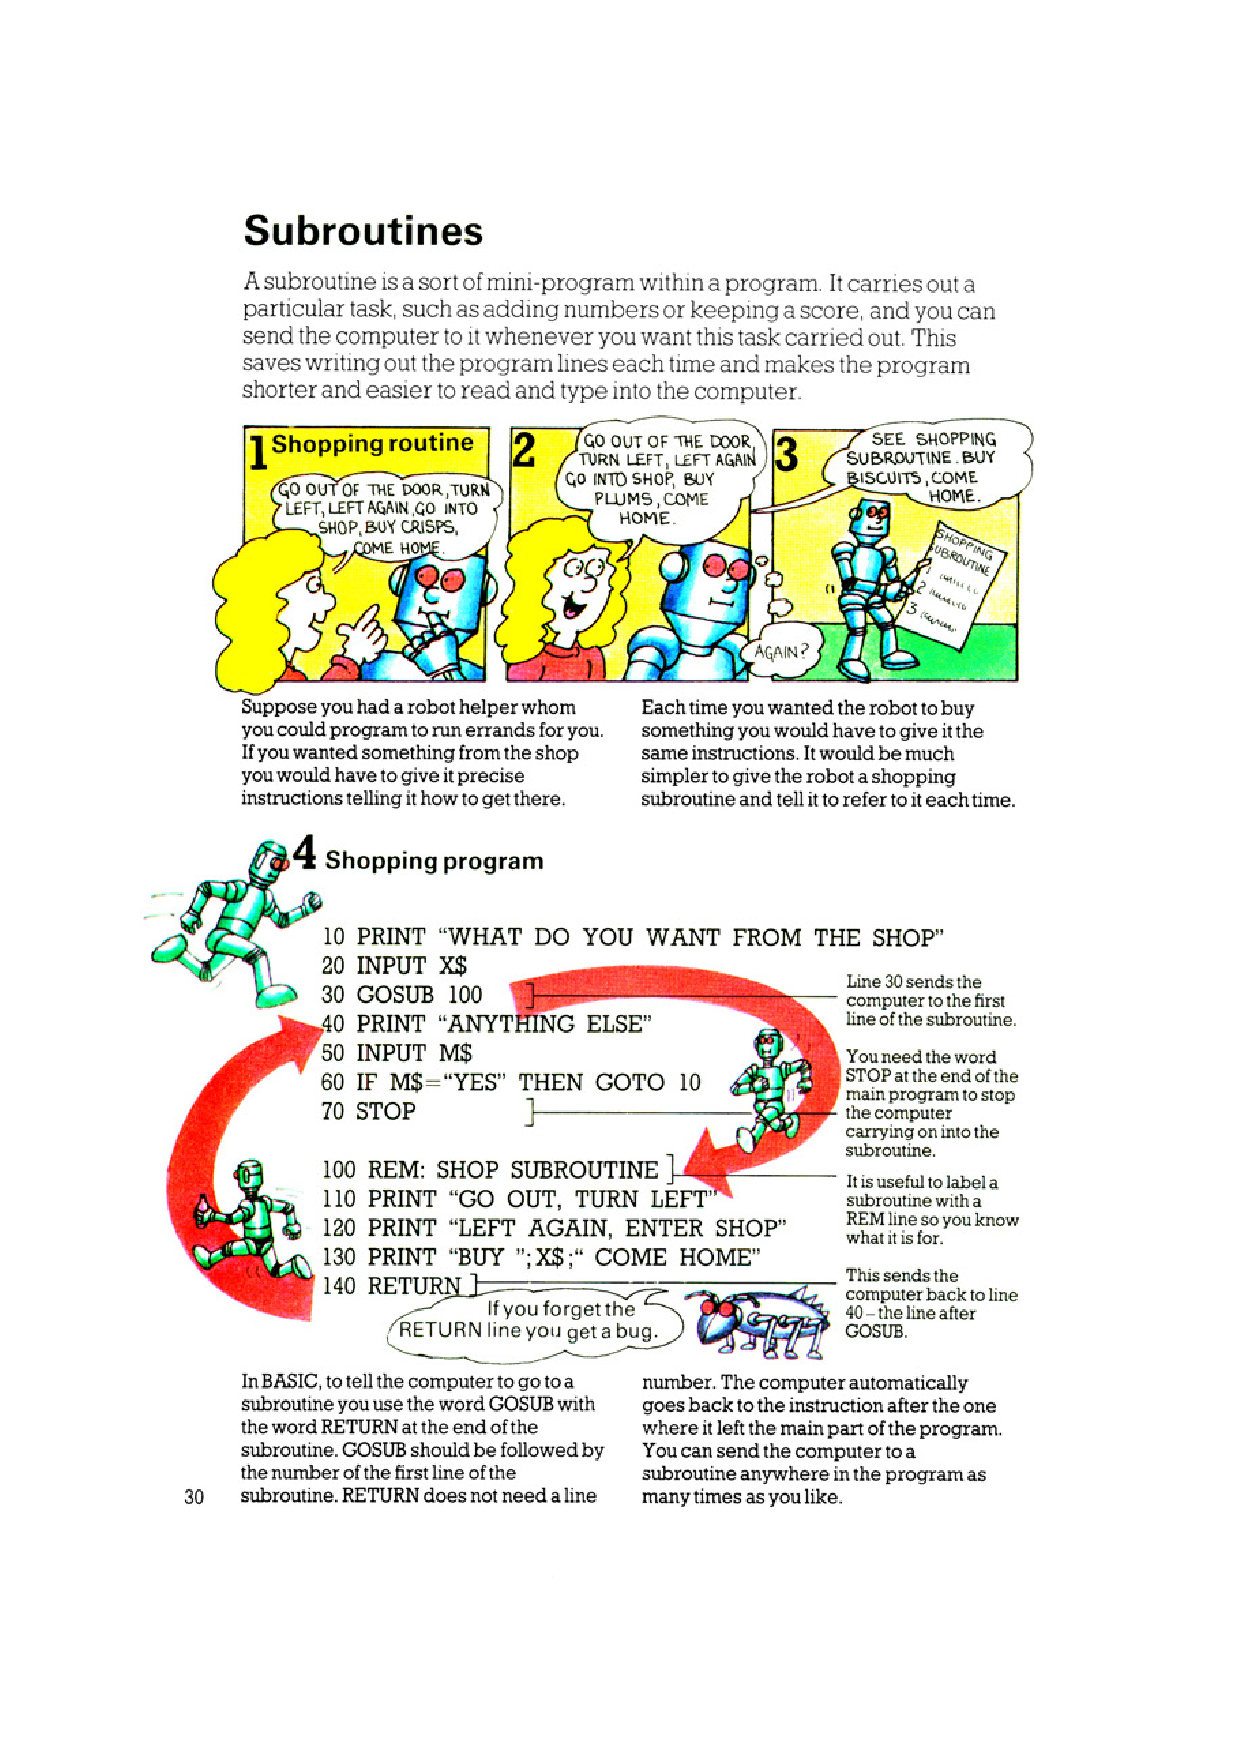
\includegraphics[height=\textheight]{subroutines}
\end{frame}

\begin{frame}{Basic Workflow}
	\begin{enumerate}
		\item Fork the official course repository on GitHub into your own account
		\item Clone your forked repository to your local computer
		\item Work on exercises in your own computer
		\item Push changes back to your fork on GitHub
		\item Open pull requests to merge your work to the main course repository
	\end{enumerate}
\end{frame}

\section{Fortran}

\begin{frame}
	\centering
	\Huge \textbf{Introduction to Fortran}
\end{frame}

% Fortran overview
\begin{frame}{Fortran}
	\begin{itemize}
		\item Compiled programming language (vs. interpreted like Python)
		\item Developed in the 1950s for scientific computing
		\item Very good for numerically heavy problems in physics
		\item Not really good for much else… but works well together with Python!
		\item Major versions: FORTRAN 77, Fortran 90/95, 2003, 2008, 2018, 2023
	\end{itemize}
\end{frame}



\begin{frame}{Compiled vs Interpreted Languages}
	\begin{columns}[T]
		\column{0.48\textwidth}
		\textbf{Compiled (Fortran, C, C++)}
		\begin{itemize}
			\item Source $\to$ machine code via compiler
			\item Produces executable before running
			\item Optimised for target CPU
			\item Requires a compiler
		\end{itemize}

		\column{0.48\textwidth}
		\textbf{Interpreted (Bash, Python, R, Matlab)}
		\begin{itemize}
			\item Source executed by an interpreter at run time
			\item No separate compilation step
			\item Requires interpreter to run
		\end{itemize}
	\end{columns}
\end{frame}


\begin{frame}{Performance}
	\begin{columns}[T]
		\column{0.48\textwidth}
		\textbf{Compiled}
		\begin{itemize}
			\item Very fast execution
			\item Runs as native machine code, with no interpreter in between
			\item Speed still depends on compiler optimisation (e.g., \texttt{-O2}, \texttt{-O3})
		\end{itemize}

		\column{0.48\textwidth}
		\textbf{Interpreted}
		\begin{itemize}
			\item Slower due to interpreter overhead
			\item Pure-Python loops are often 10--100$\times$ slower than compiled code
			\item NumPy, Numba, and JAX can close most of the gap
		\end{itemize}
	\end{columns}
\end{frame}


\begin{frame}{Development Speed}
	\begin{columns}[T]
		\column{0.48\textwidth}
		\textbf{Compiled}
		\begin{itemize}
			\item Slower cycle: edit $\to$ compile $\to$ run
			\item More boilerplate code
		\end{itemize}

		\column{0.48\textwidth}
		\textbf{Interpreted}
		\begin{itemize}
			\item Rapid iteration: edit $\to$ run
			\item Shorter programs, easier syntax
		\end{itemize}
	\end{columns}
\end{frame}

\begin{frame}{Portability}
	\begin{columns}[T]
		\column{0.48\textwidth}
		\textbf{Compiled}
		\begin{itemize}
			\item Standard-conforming source code is portable
			\item \ldots but the executable must be rebuilt for each OS and CPU architecture
		\end{itemize}

		\column{0.48\textwidth}
		\textbf{Interpreted}
		\begin{itemize}
			\item The code can be run with any setup (if the interpreter exists)
		\end{itemize}
	\end{columns}
\end{frame}


\begin{frame}{Error Handling}
	\begin{columns}[T]
		\column{0.48\textwidth}
		\textbf{Compiled}
		\begin{itemize}
			\item Many errors caught at compile time
			\item Type mismatches, missing variables flagged early
			\item Some errors still happen at run time (e.g., out-of-bounds array access, which is \emph{not} checked by default)
			\item During development, compile with \texttt{-Wall -fcheck=all}
		\end{itemize}

		\column{0.48\textwidth}
		\textbf{Interpreted}
		\begin{itemize}
			\item Errors appear at runtime
			\item Flexible, but can fail late
		\end{itemize}
	\end{columns}
\end{frame}


\begin{frame}{Typical Use Cases}
	\begin{columns}[T]
		\column{0.48\textwidth}
		\textbf{Compiled}
		\begin{itemize}
			\item Heavy numerical simulations
			\item High-performance computing
			\item Long-running production code
		\end{itemize}

		\column{0.48\textwidth}
		\textbf{Interpreted}
		\begin{itemize}
			\item Data analysis and exploration
			\item Rapid prototyping
			\item Teaching, scripting, glue code
		\end{itemize}
	\end{columns}
\end{frame}


\begin{frame}[fragile]{Fortran: First Steps}
		\begin{columns}[T]
		\column{0.48\textwidth}
		\begin{itemize}
		\item Program code inside a \texttt{program ... end program} block
		\item Always use \texttt{implicit none}
		\item Simple printing: \texttt{print *, ...}
		\end{itemize}
		\column{0.48\textwidth}
\begin{lstlisting}[language=Fortran]
program hello
  implicit none
  print *, "Hello world!"
end program hello
\end{lstlisting}
	\end{columns}
\end{frame}

\begin{frame}[fragile]{Compiling Fortran}
	\begin{itemize}
		\item Source code file $\to$ executable program
		\item Free compilers: GNU \texttt{gfortran}, LLVM \texttt{flang}, Intel \texttt{ifx}, NVIDIA \texttt{nvfortran}, AMD AOCC
		\item Vendor compilers optimise for their own hardware, but \texttt{gfortran} is usually enough (and is what we use)
	\end{itemize}
\begin{lstlisting}[language=bash]
$ gfortran -o hello hello.f90
$ ./hello
\end{lstlisting}
\end{frame}

\begin{frame}{Fortran Source Files}
	\begin{itemize}
		\item Use suffix \texttt{.f90} for modern Fortran
		\item Avoid version-specific suffixes (\texttt{.f03}, \texttt{.f08}, …)
	\end{itemize}
\end{frame}


\section{Version Control}
\begin{frame}
	\centering
	\Huge \textbf{Version Control}
\end{frame}

\begin{frame}{Version Control: What It Is and Why We Need It}
	\begin{itemize}
		\item Tracks changes in code, documents, and data
		\item Allows you to:
		\begin{itemize}
			\item Revert to earlier versions
			\item Compare changes over time
			\item Work on features without breaking main code
		\end{itemize}
		\item Essential for collaboration
		\item Prevents the ``final\_v2\_really\_final.f90'' problem
	\end{itemize}
\end{frame}

\begin{frame}{Version Control Concepts}
	\begin{itemize}
		\item \textbf{Repository}: a project's files plus their complete history
		\item \textbf{Commit}: snapshot of project at a given time
		\item \textbf{Branch}: parallel line of development
		\item \textbf{Merge}: combine changes from different branches
		\item \textbf{Remote}: another copy of the repository (e.g., on GitHub) that you exchange commits with
	\end{itemize}
	\vspace{0.5em}
	Git is by far the most widely used system today. Older systems, such as Subversion (SVN) and Mercurial, are still found in some older projects.
\end{frame}


\section{Version Control with Git}
\begin{frame}
	%\frametitle{What is Git?}
	\begin{block}{What is Git?}
		\textbf{Distributed Version Control System (VCS)}
		\begin{itemize}
			\item Tracks changes in the source code and helps coordinate work among programmers.
			\item Designed to handle everything from small to very large projects quickly and efficiently.
			\item Allows multiple developers to work on a project simultaneously without overwriting each other's changes.
		\end{itemize}
	\end{block}

	\begin{block}{Distributed?}
		\justifying
		\begin{itemize}
			\item Each user has a full copy of the repository.
			\item Allows for a more flexible workflow than centralised VCSs.
			\item Committing, branching, and browsing history are fast and do not require a network connection.
		\end{itemize}
	\end{block}

\end{frame}


\begin{frame}
	\frametitle{Why Use Git?}
	\begin{itemize}
		\item \textbf{Collaboration:} Streamlines teamwork on projects.
		\item \textbf{Backup and Restore:} Safeguards code with version history.
		\item \textbf{Track History:} Allows you to see what changes were made and when.
		\item \textbf{Branching and Merging:} Supports multiple development lines.
	\end{itemize}
\end{frame}

\begin{frame}
	\frametitle{Installing Git}
	\begin{block}{Windows}
		Install via \href{https://git-scm.com/download/win}{Git for Windows}.
	\end{block}
	\begin{block}{Mac}
		Install the Xcode command-line tools with \texttt{xcode-select -{}-install}, or use Homebrew: \texttt{brew install git}.
	\end{block}
	\begin{block}{Linux}
		Install via package manager using \texttt{sudo apt install git} or equivalent.
	\end{block}
\end{frame}

\begin{frame}[fragile]
	\frametitle{Configuring Git}
	Set your username, email, and default branch name:
\begin{lstlisting}[language=bash]
$ git config --global user.name "Your Name"
$ git config --global user.email "you@example.com"
$ git config --global init.defaultBranch main
\end{lstlisting}
	\begin{itemize}
		\item The name and email are used to attribute commits to you.
		\item Use the same email as in your GitHub account so that GitHub links the commits to your profile.
		\item Without the last setting, new repositories may still start with a branch called \texttt{master} instead of \texttt{main}.
		\item The \texttt{-{}-global} flag applies settings for all repositories.
	\end{itemize}
\end{frame}

%\section{Basic Git Commands}

\begin{frame}[fragile]
	\frametitle{Initializing a Repository}
	Initialize a new Git repository in the current directory:
\begin{lstlisting}[language=bash]
$ git init
\end{lstlisting}
	\begin{itemize}
		\item Creates a new \texttt{.git} subdirectory that will store the history.
		\item Nothing is tracked yet: files must be added with \texttt{git add} and committed with \texttt{git commit}.
	\end{itemize}
\end{frame}

\begin{frame}[fragile]
	\frametitle{Checking Status}
	Check the status of your working directory and staging area:
\begin{lstlisting}[language=bash]
$ git status
\end{lstlisting}
	\begin{itemize}
		\item Shows untracked files and modified tracked files.
		\item Indicates changes that are staged for commit.
	\end{itemize}
\end{frame}

\begin{frame}
	\frametitle{How Git Tracking Works}
	\begin{itemize}
		\item \textbf{Working Directory:} Your local filesystem where you modify files.
		\item \textbf{Staging Area (Index):} A temporary area where you add changes to prepare for a commit.
		\item \textbf{Repository (History):} The database where commits are stored.
		\item \textbf{Tracking Changes:}
		\begin{itemize}
			\item Git monitors changes in tracked files.
			\item Untracked files are not monitored until added.
		\end{itemize}
		\item \textbf{Lifecycle of a File:}
		\begin{enumerate}
			\item Modify files in the working directory.
			\item Stage changes using \texttt{git add}.
			\item Commit changes to the repository with \texttt{git commit}.
		\end{enumerate}
	\end{itemize}
\end{frame}

\begin{frame}
	\frametitle{Staging vs. Committing Changes}
	\begin{itemize}
		\item \textbf{Staging Changes (\texttt{git add}):}
		\begin{itemize}
			\item Prepares selected changes for the next commit.
			\item Allows you to review and group changes.
		\end{itemize}
		\item \textbf{Committing Changes (\texttt{git commit}):}
		\begin{itemize}
			\item Records the staged changes into the repository history.
			\item Creates a new commit object with a unique ID.
			\item Includes a commit message describing the changes.
		\end{itemize}
		\item \textbf{Key Differences:}
		\begin{itemize}
			\item \textbf{Staging:} Prepares changes, but does not save them to history.
			\item \textbf{Committing:} Records the staged changes in the history.
		\end{itemize}
	\end{itemize}
\end{frame}

\begin{frame}[fragile]
	\frametitle{Staging Changes with \texttt{git add}}
	Add files to the staging area:
\begin{lstlisting}[language=bash]
$ git add filename
$ git add .
\end{lstlisting}
	\begin{itemize}
		\item \texttt{git add filename}: Stages a specific file.
		\item \texttt{git add .}: Stages \emph{all} changes (new, modified, and deleted files) in the current directory and its subdirectories.
		\item \textbf{Staging:} Prepares changes to be included in the next commit.
		\item Check \texttt{git status} before committing so that you do not add files by accident!
	\end{itemize}
\end{frame}

\begin{frame}[fragile]
	\frametitle{Ignoring Files with \texttt{.gitignore}}
	A \texttt{.gitignore} file lists files that Git should never track:
\begin{lstlisting}[language=bash]
# Compiled objects and modules
*.o
*.mod
# Executables
hello
*.exe
\end{lstlisting}
	\begin{itemize}
		\item Keep build products (object files, modules, executables) and large data files out of the repository.
		\item These files can always be regenerated from the source code.
		\item The \texttt{.gitignore} file itself is committed like any other file.
	\end{itemize}
\end{frame}

\begin{frame}[fragile]
	\frametitle{Committing Changes with \texttt{git commit}}
	Commit the staged changes to the repository:
\begin{lstlisting}[language=bash]
$ git commit -m "Commit message"
\end{lstlisting}
	\begin{itemize}
		\item Records a snapshot of the staging area.
		\item \textbf{Commit Message:} Describes the changes made.
	\end{itemize}
\end{frame}

\begin{frame}[fragile]
	\frametitle{Inspecting History and Changes}
\begin{lstlisting}[language=bash]
$ git log --oneline        # list commits, newest first
$ git diff                 # unstaged changes
$ git diff --staged        # staged changes (what will be committed)
$ git show <commit>        # contents of a single commit
\end{lstlisting}
	\begin{itemize}
		\item Use \texttt{git diff} before \texttt{git add} to review what you changed.
		\item Each commit is identified by a hash (e.g., \texttt{9ce14a9}); a short prefix is usually enough.
	\end{itemize}
\end{frame}


\begin{frame}
	\frametitle{Understanding Branches}
	\begin{itemize}
		\item \textbf{What is a Branch?}
		\begin{itemize}
			\item A lightweight, movable pointer to a commit that advances as you commit.
			\item Creating one is instantaneous, so branches are cheap to use.
			\item Allows you to work on different features independently.
		\end{itemize}
		\item \textbf{Why Use Branches?}
		\begin{itemize}
			\item Isolate development work without affecting the main codebase.
			\item Facilitate collaboration by allowing multiple features to be developed simultaneously.
		\end{itemize}
		\item \textbf{Default Branch:} Typically named \texttt{main} (older repositories: \texttt{master}).
	\end{itemize}
\end{frame}

\begin{frame}[fragile]
	\frametitle{Creating and Switching Branches}
	Create a new branch and switch to it:
\begin{lstlisting}[language=bash]
$ git branch new-feature
$ git switch new-feature
\end{lstlisting}
	Or combine both steps:
\begin{lstlisting}[language=bash]
$ git switch -c new-feature
\end{lstlisting}
	\begin{itemize}
		\item \texttt{git branch new-feature}: Creates a new branch named \texttt{new-feature}.
		\item \texttt{git switch new-feature}: Switches to the \texttt{new-feature} branch.
		\item \texttt{git switch -c new-feature}: Creates and switches to \texttt{new-feature} in one command.
		\item Older guides use \texttt{git checkout} (and \texttt{git checkout -b}) for the same purpose; it still works.
	\end{itemize}
\end{frame}

\begin{frame}[fragile]
	\frametitle{Merging Branches}
	Merge changes from \texttt{new-feature} branch into \texttt{main}:
\begin{lstlisting}[language=bash]
$ git switch main
$ git merge new-feature
\end{lstlisting}
	\begin{itemize}
		\item \texttt{git switch main}: Switches to the \texttt{main} branch.
		\item \texttt{git merge new-feature}: Merges \texttt{new-feature} into \texttt{main}.
		\item \textbf{Merging:} Combines changes from one branch into another.
		\item \textbf{Conflicts:} If both branches changed the same lines, Git stops and marks the conflicting lines in the files. Edit the files to resolve the conflict, then \texttt{git add} and \texttt{git commit}.
	\end{itemize}
\end{frame}

\section{Introduction to GitHub}

\begin{frame}
	\frametitle{What is GitHub?}
	\begin{itemize}
		\item \textbf{Code Hosting Platform:} Hosts Git repositories online.
		\item \textbf{Facilitates Collaboration:} Tools for team communication and coordination.
		\item \textbf{Additional Features:}
		\begin{itemize}
			\item Issue tracking.
			\item Pull requests for code reviews.
			\item Wiki pages and documentation.
		\end{itemize}
	\end{itemize}
\end{frame}

\begin{frame}
	\frametitle{Setting Up GitHub}
	\begin{itemize}
		\item \textbf{Create an Account:} Sign up at \href{https://github.com}{github.com}.
		\item \textbf{Enable Two-Factor Authentication (2FA):} Required by GitHub for code contributors (e.g., use an authenticator app).
		\item \textbf{Set Up Authentication for Git:}
		\begin{itemize}
			\item Your GitHub password \emph{cannot} be used for \texttt{git push} or \texttt{git pull}.
			\item Use an SSH key (next slide) and the SSH repository URLs (\texttt{git@github.com:...}).
			\item Alternative: the GitHub CLI, \texttt{gh auth login}, sets everything up interactively.
		\end{itemize}
	\end{itemize}
\end{frame}

\begin{frame}[fragile]
	\frametitle{Setting Up an SSH Key}
\begin{lstlisting}[language=bash]
# 1. Generate a key pair (press Enter to accept the default location)
$ ssh-keygen -t ed25519 -C "you@example.com"

# 2. Print the public key and copy it
$ cat ~/.ssh/id_ed25519.pub

# 3. On GitHub: Settings > SSH and GPG keys > New SSH key, paste the key

# 4. Test the connection
$ ssh -T git@github.com
\end{lstlisting}
	\begin{itemize}
		\item Only the \emph{public} key (\texttt{.pub}) is shared. Never share the private key.
	\end{itemize}
\end{frame}


\begin{frame}[fragile]
	\frametitle{Connecting a Local Repository to GitHub}
	Add a remote repository and push changes:
\begin{lstlisting}[language=bash]
$ git remote add origin git@github.com:username/repo.git
$ git push -u origin main
\end{lstlisting}
	\begin{itemize}
		\item \texttt{git remote add origin}: Links your local repo to GitHub under the name \texttt{origin}.
		\item \texttt{git push -u origin main}: Pushes your local \texttt{main} branch to GitHub.
		\item \textbf{The \texttt{-u} Flag:} Makes \texttt{origin/main} the upstream of your local \texttt{main}, so that a plain \texttt{git push} or \texttt{git pull} works afterwards.
		\item A repository created with \texttt{git clone} already has \texttt{origin} set up.
	\end{itemize}
\end{frame}

\begin{frame}[fragile]
	\frametitle{Pushing and Pulling}
\begin{lstlisting}[language=bash]
$ git push      # send your new commits to the remote
$ git pull      # fetch new commits from the remote and merge them
\end{lstlisting}
	\begin{itemize}
		\item \texttt{git push} is rejected if the remote has commits you do not have: \texttt{git pull} first, then push again.
		\item Pull regularly to avoid large merge conflicts.
	\end{itemize}
\end{frame}

\begin{frame}
	\frametitle{Collaborating on GitHub}
	\begin{itemize}
		\item \textbf{Forking Repositories:} Create a personal copy of someone else's project \emph{on GitHub}.
		\item \textbf{Cloning Repositories:} Download a repository to your local machine.
		\item \textbf{Pull Requests:} Propose changes to a repository.
		\item \textbf{Code Reviews:} Collaboratively review code changes before merging.
		\item \textbf{Issue Tracking:} Report bugs or request features.
	\end{itemize}
\end{frame}

\begin{frame}[fragile]
	\frametitle{The Fork Workflow}
	\begin{itemize}
		\item \textbf{upstream}: the original course repository (\texttt{hpparvi/ull\_tp\_2627})
		\item \textbf{origin}: your fork on GitHub (\texttt{your-username/ull\_tp\_2627})
		\item \textbf{local}: the clone on your computer
	\end{itemize}
	You push to \texttt{origin} and open pull requests from \texttt{origin} to \texttt{upstream}. To get new course material, add the upstream remote once and pull from it:
\begin{lstlisting}[language=bash]
$ git remote add upstream https://github.com/hpparvi/ull_tp_2627.git
$ git pull upstream main    # get the latest course material
$ git push origin main      # update your fork on GitHub
\end{lstlisting}
	Alternatively, use the \textbf{Sync fork} button on your fork's GitHub page and then \texttt{git pull}.
\end{frame}

\section{Best Practices and Conclusion}

\begin{frame}
	\frametitle{Best Practices}
	\begin{itemize}
		\item \textbf{Write Meaningful Commit Messages:} Clearly describe what changes were made.
		\item \textbf{Keep Commits Small and Focused:} Easier to review and understand.
		\item \textbf{Regularly Pull Updates:} Keep your local repository up-to-date with the remote.
		\item \textbf{Use Branches for New Features:} Isolate development work.
		\item \textbf{Do Not Commit Build Products:} Use \texttt{.gitignore} for object files, modules, and executables.
		\item \textbf{Avoid Committing Sensitive Information:} Don't commit passwords or API keys. Deleting the file in a later commit does \emph{not} remove it from the history, so treat a committed secret as leaked and change it.
	\end{itemize}
\end{frame}

\section{Exercises}

\begin{frame}{Preliminaries}
	\begin{columns}[T]
		\column{0.48\textwidth}
		\begin{block}{Setup a Fortran Compiler}
			\begin{itemize}
				\item Optional: set up a Conda environment
				\item Install gfortran
				\item Optional: install VSCode or another IDE
			\end{itemize}
		\end{block}
		\column{0.48\textwidth}
		\begin{block}{Setup Git \& GitHub}
			\begin{itemize}
				\item Install and configure Git (if not already done)
				\item Set up a GitHub account with 2FA
				\item Set up an SSH key and add it to GitHub
			\end{itemize}
		\end{block}
	\end{columns}
\end{frame}


\begin{frame}[fragile]{Preliminaries}
	\begin{block}{Setup Course}
	\begin{itemize}
	 \item On GitHub: click ``Fork'' on the course repository page: \\ \url{https://github.com/hpparvi/ull_tp_2627}
	 \item On your computer: clone your fork
\begin{lstlisting}[language=bash]
$ git clone git@github.com:your-username/ull_tp_2627.git
$ cd ull_tp_2627
\end{lstlisting}
	\item Add the course repository as \texttt{upstream} and verify your remotes
\begin{lstlisting}[language=bash]
$ git remote add upstream https://github.com/hpparvi/ull_tp_2627.git
$ git remote -v
\end{lstlisting}
	\end{itemize}
	\end{block}
\end{frame}

\begin{frame}{First Exercise}
	Follow the ``First steps'' in \texttt{students/README.md}:
	\begin{enumerate}
		\item Create your own directory \texttt{students/<initials>} (e.g., \texttt{students/ph})
		\item Create the subdirectories \texttt{sandbox/l01}, \texttt{course\_exercise\_1}, and \texttt{course\_exercise\_2}
		\item Add empty \texttt{README.md} files to the course exercise directories
		\item Add your name and directory to the table in \texttt{students/README.md}
		\item Stage, commit, and push the changes to your fork
		\item On GitHub, open a pull request to the course repository
	\end{enumerate}
\end{frame}

%\section{Exercises}
%% Exercises
%\begin{frame}{Exercises}
%  \begin{enumerate}
%    \item Modify the “Hello world” program to print it $n$ times,
%          where $n$ is read from the terminal.
%    \item Write a program that prints factorials $n!$ from 0 to $n$.
%    \item Write a program that prints $r!$ where $r$ is a positive
%          real number read from the terminal.
%  \end{enumerate}
%\end{frame}

\end{document}
